\documentclass[a4paper, 12pt, oneside]{article}
\usepackage{graphicx}
\begin{document}

\begin{titlepage} % Suppresses headers and footers on the title page

	\centering % Centre everything on the title page
	
	\scshape % Use small caps for all text on the title page
	
	\vspace*{\baselineskip} % White space at the top of the page
	
	%------------------------------------------------
	%	Title
	%------------------------------------------------
	
	\rule{\textwidth}{1.6pt}\vspace*{-\baselineskip}\vspace*{2pt} % Thick horizontal rule
	\rule{\textwidth}{0.4pt} % Thin horizontal rule
	
	\vspace{0.75\baselineskip} % Whitespace above the title
	
	{\LARGE Consultant Tracker\\Architectural Design} % Title
	
	\vspace{0.75\baselineskip} % Whitespace below the title
	
	\rule{\textwidth}{0.4pt}\vspace*{-\baselineskip}\vspace{3.2pt} % Thin horizontal rule
	\rule{\textwidth}{1.6pt} % Thick horizontal rule
	
	\vspace{2\baselineskip} % Whitespace after the title block
	
	
	%------------------------------------------------
	%	Editor(s)
	%------------------------------------------------
	
	Edited By
	
	\vspace{0.5\baselineskip} % Whitespace before the editors
	
	{\scshape\Large Sibekezelo Mamba 16095414 \\ Johan de Waal 16155140 \\ Stephen Munro 16024479\\ Hulisani Mudimeli 			16073364 \\ Ngonidzashe Mujuru 16285256  \\ Tatenda Mafunga 16094965\\} % Editor list
	
	\vspace{0.5\baselineskip} % Whitespace below the editor list
	
	\textit{University of Pretoria \\2018} % Editor affiliation
	
	\vfill % Whitespace between editor names and publisher logo
	
\end{titlepage}

\newpage
\tableofcontents
\newpage


\pagenumbering{arabic}

\section{Introduction}
The Consultant Tracker application is a Human-Resource system. The application will facilitate easy tracking of resource utilisation and also comparisons between allocated and actual resources spent on each project.
\subsection{Purpose}
The purpose of this document is to provide a detailed overview of the software product and its goals. It describes the user interface, hardware and software requirements.

\newpage
\section{Overall Description}
 
\subsection{Product Perspective}
The system will run as both as mobile and desktop web application. Both versions will have the same functionalities, the mobile web application is useful for quick on the go use cases such as viewing progress and feedback.
\subsubsection{System Interface}
The system will make use of a web-based Front-end that sends and receives data using Java Persistance API(JPA) to and from a hosted server.  The sever will have access to external database from which it can retrieve or store data.

\subsubsection{User Interfaces}
The interface should be easy to use and intuitive. Shown below is our prototype interface.
\begin{figure}[h!]
  \centering
  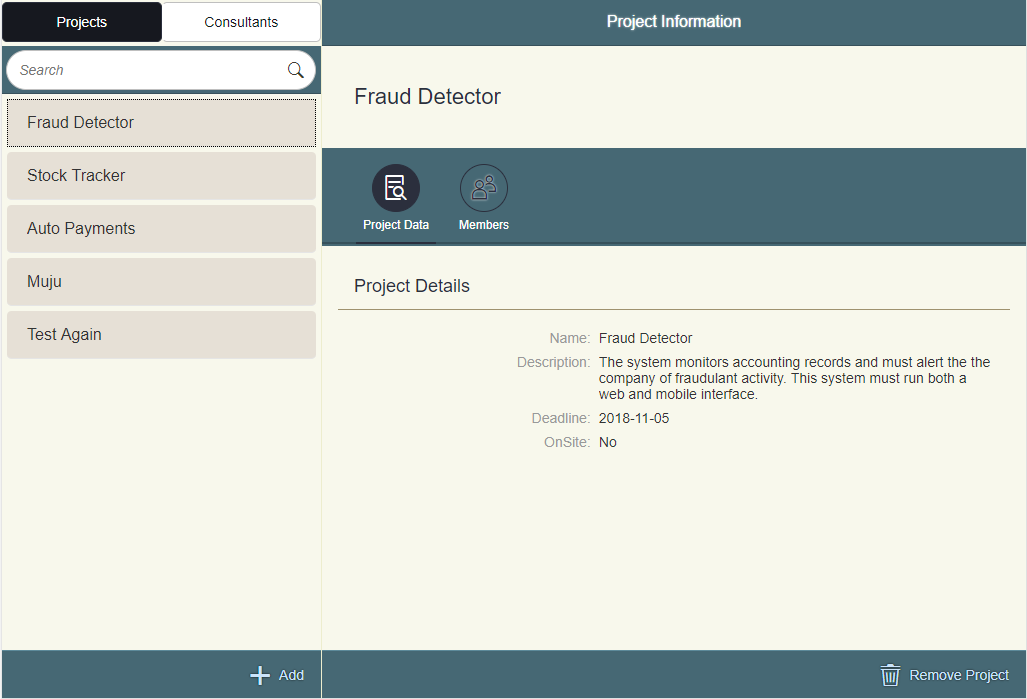
\includegraphics[width=\linewidth]{images/viewProject.PNG}
  \caption{View Project}
  \label{fig:sfig1}
\end{figure}

\begin{figure}[h!]
  \centering
  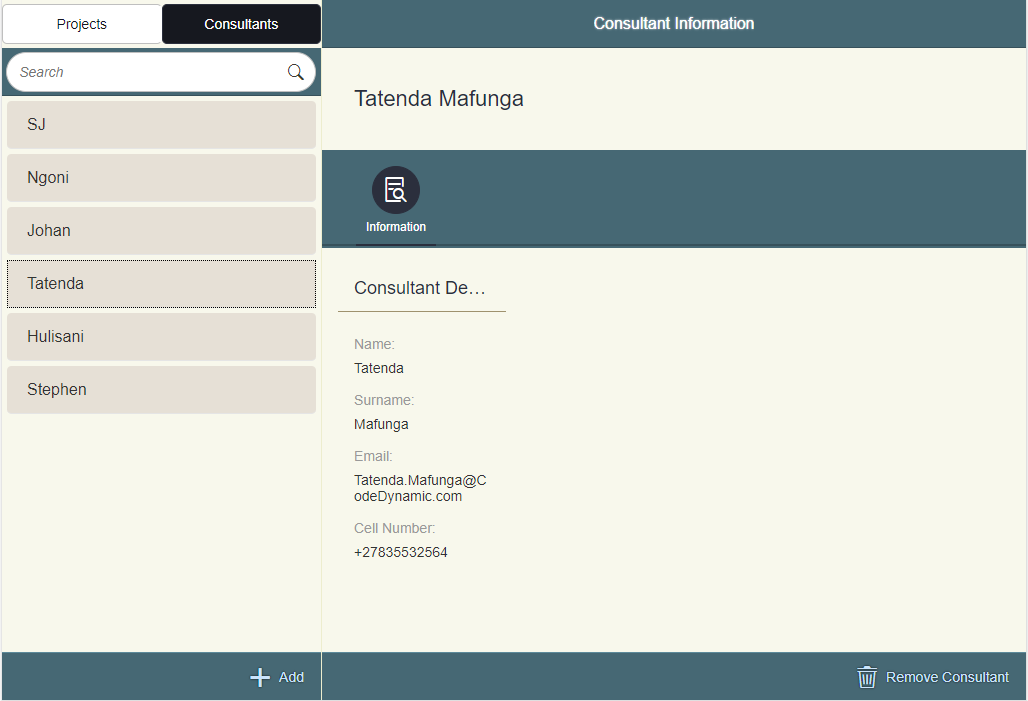
\includegraphics[width=\linewidth]{images/viewConsultant.PNG}
  \caption{View Consultant}
  \label{fig:sfig1}
\end{figure}

\subsubsection{Hardware Interface}
\begin{itemize}
	\item As the Front-end is web-based, it can be run on any device that has an internet connection and can browse the web.
	\item The server will be hosted on a computer which will be maintained to ensure that the server is always running or a company that provide hosting services can be used.
	\item The database that will be used to store the data for the application can make use of a computer that is maintained to host it or use a company that provide hosting services.
\end{itemize}
\subsubsection{Communication Interfaces}
The system requires HTTP to communicate with server. The system can be configured to be accessed via any available port. The system is accessible through all popular web browsers that interact with HTML pages.

\section{Specific Requirements}

\subsection{External interface requirements}
The system will use MYSQL database and JDBC connector to communicate with the database.

\subsection{Functional Requirements}
The actions/functions depend on the users' permissions.The users of the consultant tracker system are divided into two groups, namely,  an administrator and a consultant. The administrator group can perform all actions in the consultant group but not vice versa. 
Functions include:

\subsubsection{Login}
This allows the user to enter into the application. The user is required to provide username and password. After authentication, a user will have access to the main menu. The availability of specific functions will depend on the users' permissions.

\subsubsection{Create Project}
Allows an administrator user to log new projects and information related to that specific project.

\subsubsection{View Project}
Allows an administrator user to view all projects and the respective details currently in progress. A consultant user will only be able to view projects they have been assigned to.

\subsubsection{View and rate team members}
Allows a  consultant to view team members that he or she will be working with. At the end of a project, a consultant must be able to rate the performance of the team members. Ratings will remain anonymous, but only visible to an administrator user.

\subsubsection{Feedback}
Allows a consultant user to log any issues encountered and also allows the administrator user to view and respond accordingly.

\subsubsection{Notification subsystem}
The consultant must be notified be the system when they are assigned to a new project, as well as be notified when the allocated time is nearly reached.

\subsection{Non-functional Requirements}
The non-functional requirements will specify the limitations of the system. 

\subsubsection{Performance}
The system is expected to be responsive even under a high load (multiple users making requests).

\subsubsection{Security}
The system must be able to differentiate between the types of users. From this, the system will be able to grant specific functions to users, thus protecting the data from possible corruption caused by unauthorized actions by users.

\subsubsection{Software Quality Assurance}

\begin{itemize}
	\item \textbf{Reliability}\\ The system shall perform all its stated functions consistently. Computations of utilisation and any date related functions will be accurate.
	\item \textbf{Robustness}\\The system will be designed to work on any device which has a browser. The system must be 		data efficient so that it can work even though there are poor internet connection speeds. The presentation layer will be 		created knowing that the system will run on different devices, with different processing capabilities, that it should be kept as 		power efficient as possible to support all the devices the system can run on.
	\item \textbf{Availability}\\The system should be always available during the hours it is most popular. Any maintenance 			where the system needs to be offline should be done outside these identified times. The geographical location of the server 		must also not affect the availability of the system.
	\item \textbf{Efficiency}\\ The system will be data efficient so that it does not waste any user’s data.
	\item \textbf{Portability}\\A responsive JavaScript framework will be used for making the application so that it can run on 		different platforms using one codebase.
	\item \textbf{Maintainability}\\The code should be built modularly, such that independent parts can function independently of 	one another. Common coding styles should be utilised.
	
\end{itemize}

\subsection{Assumptions and Dependencies}
It is assumed that the application may be used on mobile phones. Although the product can be used on desktops, the product will be designed in a way that best suits mobile user’s needs.

\newpage
\section{Use cases}
\subsection{Create project}
This is a main function of the adminstrator. The administrator must
\begin{itemize}
	\item enter project details which also include client details.
	\item assign consultants to a project.
\end{itemize}
The use case diagram is given below.
\\
\begin{figure}[h!]
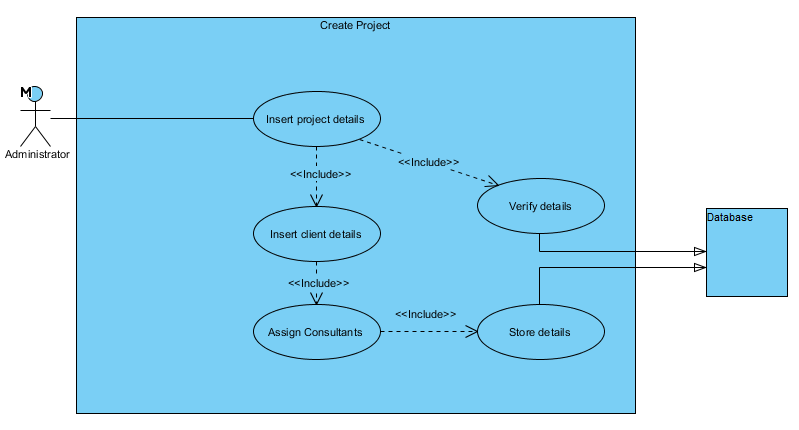
\includegraphics[width = \linewidth]{images/createProjectUCD.png}
	\caption{Create project use case diagram}
\end{figure}
\newpage
 The following sequence diagram shows the interaction between an administrator and the system interface. 
\begin{figure}[h!]
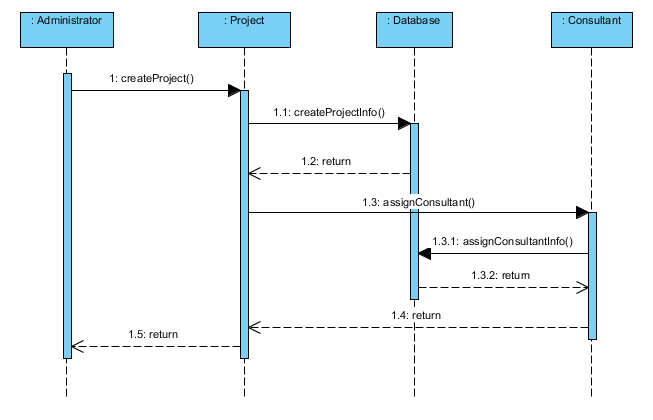
\includegraphics[width = \linewidth]{images/createProject.png}
	\caption{Create project sequence diagram}
\end{figure}

\subsection{Create consultant}
The admnistrator must be able to create a consultant account. The following image shows the use case diagram.
\begin{figure}[h!]
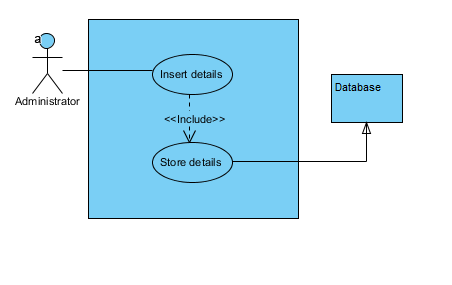
\includegraphics[width = 70mm, scale = 0.8]{images/createConsultant.png}
	\caption{Create consultant use case diagram}
\end{figure}

\subsection{Notification subsystem}
The system must notify a consultant once they are assigned to a project. The following image shows the use case diagram.
\begin{figure}[h!]
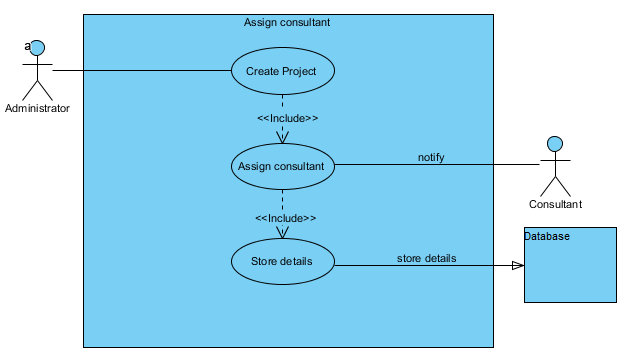
\includegraphics[width = \linewidth]{images/notificationSubsystem.png}
	\caption{Notification use case diagram}
\end{figure}
\end{document}